\documentclass[10pt]{beamer}
\usepackage{xeCJK}
\usepackage{graphicx}
\usepackage{booktabs}
\usepackage{listings}
\usepackage{multirow}
\usepackage{mathtools}
\usepackage{ulem}
\usefonttheme[onlymath]{serif}
\usetheme{metropolis}
\begin{document}
	\title{杂题水讲}
	\date{\today}
	\author{huhao}
	\maketitle
	\clearpage
	\begin{frame}
		\frametitle{CF1007 C. Guess two numbers}
		交互,两个数$a,b\in[1,10^{18}]$,你每次可以询问$x,y$,会根据条件回答(满足多个只会回答一个):
		\begin{enumerate}
			\item $x<a$
			\item $y<b$
			\item $x>a$或$y>b$
		\end{enumerate}
		你询问$x=a,y=b$时通过此题,次数限制$600$。
	\end{frame}
	\clearpage
	\begin{frame}
		\frametitle{solution (*3000)}
	
		显然,一开始满足所有询问的是一个正方形,然后若干次询问后变为一个长方形或一个L型,二分求解是$O(\log^2)$的。

		注意到有些询问二分的话对面积的消减比较小,可以在$0.8$处询问,这样可以让常数变得比较小,足以通过。
	
	\end{frame}
	\clearpage
	\begin{frame}
		\frametitle{CF1491 H. Yuezheng Ling and Dynamic Tree}
		给定$n-1$个数$f_{2\dots n}$,有两个操作(共$q$次):
		\begin{itemize}
			\item 给定$l,r,x$,令$f_{l\dots r}$减去$x$,并对$1$取较大值。
			\item 给定$u,v$,将$i,f_i$连边,形成$1$作为根的树,求$u,v$的lca。
		\end{itemize}
		$n,q\le 10^5$,1.5s。
	\end{frame}
	\clearpage
	\begin{frame}
		\frametitle{solution (*3400)}
	
		似乎没有好的$O(n~\mathrm{poly}(\log))$做法,考虑$O(n^{1.5})$。

		lca可以$O(\sqrt n)$求,不妨记两个数组:$f,F$,$f$是父亲,$F$是一个祖先。

		分为$\sqrt n$块,同时记$F$为不在同一块内的最深的祖先,不难发现求lca是$O(\sqrt n)$的。

		考虑对一整个块求$F$是$O(\sqrt n)$的,这个过程记为$1$次build。

		修改时,对两个散块进行build,复杂度是$O(q\sqrt n)$的。

		考虑到每一个块,如果对整块修改了$\sqrt n$次,那么$F=f$,就只要维护$f$了。

		均摊下来,一共进行$\sqrt n\times \sqrt n=n$次build,总复杂度$O((n+q)\sqrt n)$。
	
	\end{frame}
	\clearpage
	\begin{frame}
		\frametitle{CF1548 E. Gregor and the Two Painters}
	
		给定$n,m,a_{1\dots n},b_{1\dots m},x$,生成一个$n\times m$的黑白矩阵,$(i,j)$为黑当且仅当$a_i+b_j\le x$。
		
		求黑色连通块数。

		$n,m,a,b\in [1,200000]$。
	
	\end{frame}
	\clearpage
	\begin{frame}
		\frametitle{solution (*3400)}
	
		对于一个连通块只在$a_i+b_j$最小的格子处统计,相等统计$i,j$最大的。

		如果一个格子$(i,j)$所在连通块$(x,y)$被统计到,一定有$(i,y)$或$(x,j)$的值大于$(i,j)$,且与$(i,j)$联通。

		不难发现,可以得到$n+m$个区间$B_{1\dots n},A_{1\dots m}$,$(i,j)$被统计当且仅当$a_i\in A_j,b_j\in B_i$,扫描线+简单数据结构维护即可。
	
	\end{frame}
	\clearpage
	\begin{frame}
		\frametitle{CF566 C. Logistical Questions}
	
		给定一棵树,点边均有权,定义距离为边权和的$1.5$次方,求带权重心。

		$n\le 2\times 10^5$。
	
	\end{frame}
	\clearpage
	\begin{frame}
		\frametitle{solution (*3000)}
	
		类似普通重心的求法,注意到$x^{1.5}$是凸函数,可能有正确性?

		只要每条路径都满足那就是满足的,也就是说只要证明下面函数是凸的即可:

		$$
		f(x)=\sum_i q_i|x-p_i|^{1.5}
		$$

		即

		$$
		f''(x)=\sum_i q_i\dfrac{0.75}{\sqrt{|x-p_i|}}\ge 0
		$$

		这是$O(n^2)$的,用点分治就只要移动$\log$次了。

		但是每次都要算每个儿子的值,发现只有一个方向是可能减少的(因为是凸的),求导求出哪个方向即可。

		复杂度$O(n\log n)$。

	\end{frame}
	\clearpage
	\begin{frame}
		\frametitle{CF1237 G. Balanced Distribution}
	
		$n$个位置,每个位置有些球,环形排列,每次可以将相邻$m$个位置的球任意分配。

		求让所有位置球一样多的最小次数。
	
	\end{frame}	
	\clearpage
	\begin{frame}
		\frametitle{solution(*3500)}
	
		考虑$k=2$怎么做,就是序列上的方案绕环若干圈。

		枚举绕的圈数,然后简单统计次数即可。
	
	\end{frame}
	\clearpage
	\begin{frame}
		\frametitle{IOI2021 dungeons}
	
		\url{https://loj.ac/p/3527}
	
	\end{frame}
	\clearpage
	\begin{frame}
		\frametitle{solution}
	
		不难发现,到一个点$u$,且战败,然后经过若干次再到$u$并战胜,能力值会翻倍。

		只要能快速找环就行了。

		可以给能力值按$2$的次幂分层并倍增处理,在$[2^i,2^{i+1})$层,每个点存一下走$2^j$步,且没有战胜且能力值不小于$2^i$的位置。

		查询时倍增查询即可,复杂度$O((n+q)\log^2n)$。
	
	\end{frame}







	
	% 下面是拼凑以前的课件








	
	\begin{frame}
		\frametitle{CF1208G Polygons}
		\par 给定$n,k$
		\par 你需要构造$k$个有相同外接圆的多边形,使得边数在$3\sim n$间且边数两两不同
		\par 你可以任意旋转它们,求它们与这个外接圆的最少交点数
		\par 下面是$n=6,k=2$(边数为$3,6$)的一种方案
		\par 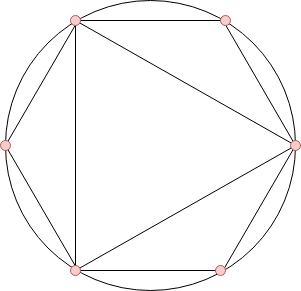
\includegraphics[width = 0.4\textwidth]{1.png}
		\par $k\le n-2,n\le 10^6$
	\end{frame}
	\clearpage
	\begin{frame}
		\frametitle{solution(*2800)}
		显然,这些多边形会有一个共同的交点

		于是,发现如果$u|v$,那么$u$肯定比$v$先选

		并且如果所有$u|v$都选了,那么$v$的代价为$\phi(v)$

		按$\phi$排序后从小到大选即可,当然因为没有$2$边形,特判掉即可
	\end{frame}
	\clearpage
	\begin{frame}
		\frametitle{IOI2019排列鞋子}
		\par 给定长度为$2n$的数组$S$
		\par 一个数组合法当且仅当$\forall i,\exists j>0,a_{2i-1}=-j,a_{2i}=j$
		\par 每次可以交换相邻两个数,求最少交换次数
		\par $n\le 10^5,1\le |a_i|\le n$
	\end{frame}
	\clearpage
	\begin{frame}
		\frametitle{solution}
		做$n$次,每次把与当前序列中第一个配对的移到前面来(有相同值就取第一个),然后删除

		考虑证明

		显然,当$S_i$有相同的时候,贪心从前往后配对(并给新标号)是对的,记$p_v$为$v$的位置

		把$i$和$−i$配对,要交换$|p_i−p_{−i}|−[p_{−i}<p_i]$次,然后在交换的过程中,对所有$j$,且$p_j$和$p_{−j}$仅有一个在$p_i$到$p_{−i}$区间内,那么它们距离减一

		于是我们从前往后配对即可,把这个过程模拟出来就是上面做法了 
	\end{frame}
	\clearpage
	\begin{frame}{Invisiable Integers}

		invisible integers是一种简单的游戏,玩家通过一些提示来猜一个由数字$1$到$9$组成的隐藏序列。每一个提示都是一个由下列规则生成的由互不相同的数字组成的序列:

		从隐藏序列中选出任意的起始位置。

		选择一个方向---向左或者向右。

		从选择的起始位置开始、以选定的方向遍历隐藏序列中的整数,将没有出现在提示中的数加在提示末尾。

		找出一个最短的长度,使得存在一个在这个长度下满足所有提示的序列。

		提示个数不大于$10$。
	\end{frame}
	\clearpage
	\begin{frame}{Solution}
	
		首先有一种简单的$O(n!\operatorname{poly}(n))$的做法:

		考虑枚举每个提示向左$L$或向右$R$,枚举出现的顺序。

		枚举$R_1$的起始位置,有用的信息只有$L_{1\dots x}$处理完了,$L_x$处理到了第$y$位。

		发现继续枚举即可,不过需要想想怎么维护和继承信息。
	\end{frame}
	\clearpage
	\begin{frame}{维护}

		考虑到向左的:
	
		$$
		\begin{aligned}
		\rm{\color{red}123}45\xrightarrow{2}&{\color{red}12}345\\
		\rm{\color{red}123}45\xrightarrow{4}&{\color{red}1234}5\\
		\rm{\color{red}123}45\xrightarrow{5}&{\color{red}123}45\\
		\rm{\color{red}123}45\xrightarrow{6}&-1\\
		\end{aligned}
		$$
		考虑到向右的:
	
		$$
		\begin{aligned}
		\rm{\color{red}123}45\xrightarrow{2}&{\color{red}123}45\\
		\rm{\color{red}123}45\xrightarrow{4}&{\color{red}1234}5\\
		\rm{\color{red}123}45\xrightarrow{5}&-1\\
		\rm{\color{red}123}45\xrightarrow{6}&-1\\
		\end{aligned}
		$$
	
	\end{frame}
	\clearpage
	\begin{frame}
		\frametitle{继承}

		向左的相当于依次插入。

		向右的有些麻烦,如果12345,在处理完12后,可以在后面接一个1345的。
		
		即是在没处理完的时候继承。
	\end{frame}
	\clearpage
	\begin{frame}{整理一下}
	
		维护信息比较简单,但是继承需要分两种:

		\begin{itemize}
			\item 向左的: 处理完$i$后,下一个是$j$,$j$的信息就是空的依次加上$i$的元素。
			\item 向右的: 处理$i$时,如果$i$依次加上$j$的元素后是整个$i$,那么可以视为处理完了$i$,然后从$j$的开头处理$j$。
		\end{itemize}
	
	\end{frame}
	\clearpage
	\begin{frame}{回到那个暴力}
	
		可以DP,记当前DP到了$i,j,k,l$,即当前处理的向左的是$i$,处理了$j$位,向右的是$k$,处理了$l$位。

		复杂度:$O(n!9^5)=O(n!)$?
	
	\end{frame}
	\clearpage
	\begin{frame}{solution}
	
		考虑到这是不是可以状压。

		有用的状态只有那个$i,j,k,l$,和每个位置是否被处理过。

		于是就可以直接优化了,有亿点细节,复杂度$O(2^n\operatorname{poly}(n))$。
	\end{frame}
	\clearpage
	\begin{frame}{Gomoku}
	
		这是一道交互题。

		五子棋是一种两个人在二维棋盘上玩的游戏。棋盘上的每个格子可以为空,放有第一名玩家的棋子(黑),或者放有第二名玩家的棋子(白),但是不能都有。初始时所有的格子都是空的。两个玩家轮流操作,从第一名玩家开始。每次操作,一名玩家可以把他的棋子放进恰好一个空格子里。首先在一行中放下五个相邻棋子的玩家获胜。一行可以是横行、竖行或对角线。

		在这个问题中,玩家们使用 $19\times 19$ 的棋盘。如果整个棋盘都放满了棋子但无人获胜,游戏平局。
	\end{frame}
	\clearpage

	\begin{frame}{Gomoku}
		第一名玩家将会使用下面的策略:第一次操作时,她会把她的棋子放到棋盘的正中间。在后面的每次操作中,她会选择一个下子后局面分数最大的位置下子。

		为了计算一个局面的分数,第一名玩家会考虑能组成胜利组合的所有地方——换句话说,棋盘上所有横行、竖行、对角线上五个连续的格子(当然,它们会互相重叠)。如果这一行同时包括了第一名玩家的棋子和第二名玩家的棋子,就无视它。如果这一行包括了恰好 $k (1\le k\le 5)$ 个第一名玩家的棋子而没有第二名玩家的棋子,给该局面的分数加上 $50^{2k−1}$。如果这一行包括了恰好 $k$ 个第二名玩家的棋子而没有第一名玩家的棋子,给该局面的分数减去 $50^{2k}$。最后,给分数加上一个 $0$ 到 $50^2−1$ 的随机数。随机数是均匀分布的。

		如果第一名玩家有多个分数相同的格子可选(因为上面提到的随机分数的原因,这是非常罕见的),第一名玩家选择 X 坐标最小的位置,如果仍有多个格子有相同的 X 坐标,就选择 Y 坐标最小的位置。

		你的任务是,写一个程序扮演第二名玩家,并打败上述的策略。
	\end{frame}
	\clearpage
	\begin{frame}{solution}
	
		如图(按字母顺序下):

		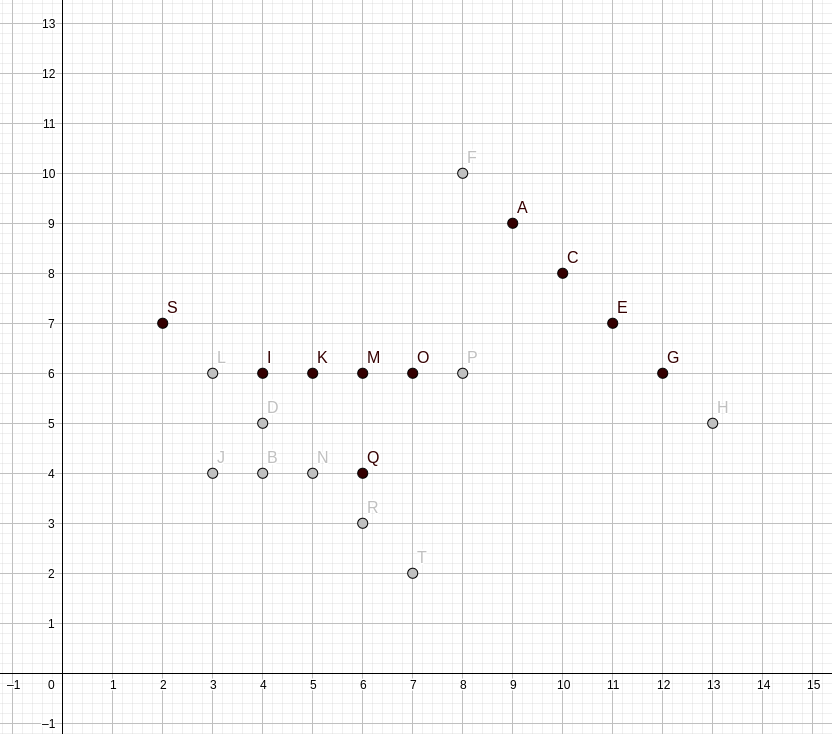
\includegraphics[width=0.8\textwidth]{2.png}

	
	\end{frame}
\end{document}